\documentclass[twocolumn]{article}
\usepackage{algorithmicx}
\usepackage{algpseudocode}
\usepackage{algorithm}
\usepackage{amsmath}
\usepackage{amssymb}
\usepackage{amsfonts}
\usepackage{stmaryrd}
\usepackage{hyperref}
\usepackage[pdftex]{graphicx}

\newcommand{\leaves}{\mathit{leaves}}
\newcommand{\branches}{\mathit{branches}}
\newcommand{\desc}{\mathit{desc}}
\newcommand{\bleft}{\mathit{left}}
\newcommand{\bright}{\mathit{right}}
\newcommand{\bbox}{\mathit{bbox}}
\newcommand{\broot}{\mathrm{root}}

\begin{document}

\section{Introduction}

\section{Background}

\section{Traversal Methods}

\begin{algorithm}
\caption{Ordered Depth First Traversal}\label{ODF}
\begin{algorithmic}[1]
\Procedure{ODF\_Traverse}{$b,r$} 
	\State $s \gets \{b\}$ 
	\State $c \gets \infty$  
	\While{$s\not=\emptyset$}
		\State $n\gets \mathit{pop}(s)$ 
		\If{$n \in \branches(b)$}
			\If{$\mathrm{intersect}(r,n.\bleft) < c$}
				\State $\mathrm{push}(s,n.\bleft)$
			\EndIf
			\If{$\mathrm{intersect}(r,n.\bright) < c$}
				\State $\mathrm{push}(s,n.\bright)$
			\EndIf
		\ElsIf{$n \in \leaves(b)$}
			\If{intersect$(r,n.\mathit{prim})<  c$}
				\State $t \gets n.\mathit{prim}$
				\State $c \gets \mathrm{intersect}(r,t)$
			\EndIf
		\EndIf
	\EndWhile
	\If{$c = \infty$}
		\State \textbf{return} \textit{null}
	\EndIf
	\State \textbf{return} $t$
\EndProcedure
\end{algorithmic}
\end{algorithm}

\begin{algorithm}
\caption{Ray Order Traversal}\label{RayOrder}
\begin{algorithmic}[1]
\Procedure{RayOrder\_Traverse}{$b,r$} 
	\State $q \gets \{\}$
			\State $\mathrm{push}(q, n.\bleft, \mathrm{intersect}(r,n.\bleft))$
	\While{$q\not=\emptyset$}
		\State $n\gets \mathit{pop}(q)$ 
		\If{$n \in \branches(b)$}
			\State $\mathrm{push}(q, n.\bleft, \mathrm{intersect}(r,n.\bleft))$
			\State $\mathrm{push}(q, n.\bright, \mathrm{intersect}(r,n.\bright))$
		\ElsIf{$n \in \leaves(b)$}
			\If{$\mathrm{intersect}(r,n.\mathit{prim}) \not= \infty$}
				\State $\mathrm{push}(q, n.\mathit{prim}, \mathrm{intersect}(r,n.\mathit{prim}))$
			\EndIf
		\ElsIf{$n \in \mathit{primitives}(b)$}
			\State \textbf{return} $n$
		\EndIf
	\EndWhile
	\State \textbf{return} \textit{null}
\EndProcedure
\end{algorithmic}
\end{algorithm}

\section{Experimental Setup}

\section{Results}
\begin{figure*}
\caption{Not bad}
\begin{tabular}{|c|c|c|c|}
\hline
Sphere & Plane & Hemisphere & Tube \\
\hline
image1 & image2 & image3 & image4 \\
\hline 
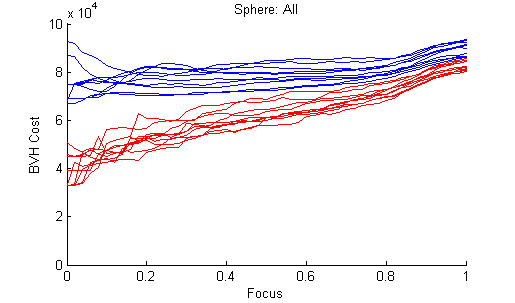
\includegraphics[scale=.3]{sphere_all.png}
&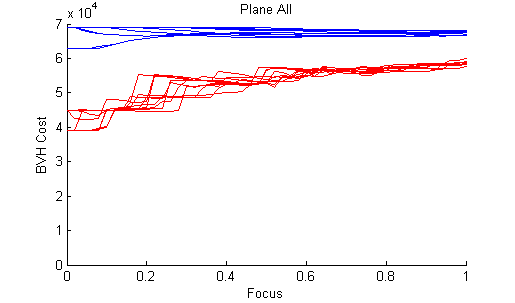
\includegraphics[scale=.3]{plane_all.png}
&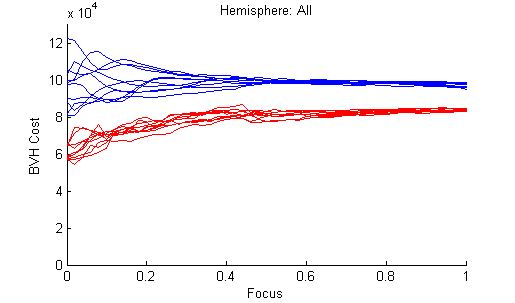
\includegraphics[scale=.3]{hemisphere_all.png}
&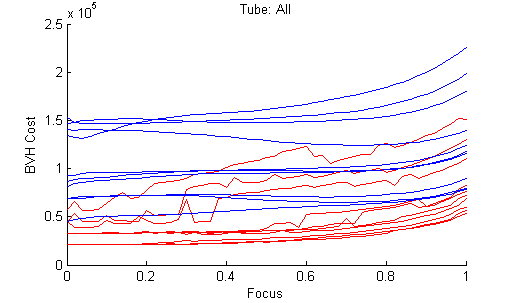
\includegraphics[scale=.3]{tube_all.png}\\
\hline
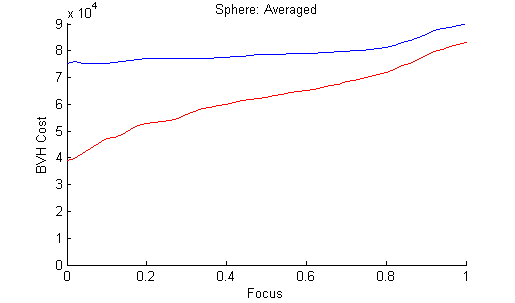
\includegraphics[scale=.3]{sphere_average.png}
&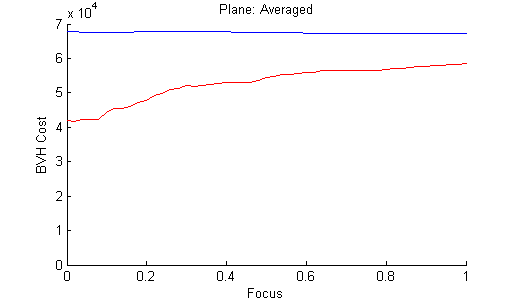
\includegraphics[scale=.3]{plane_average.png}
&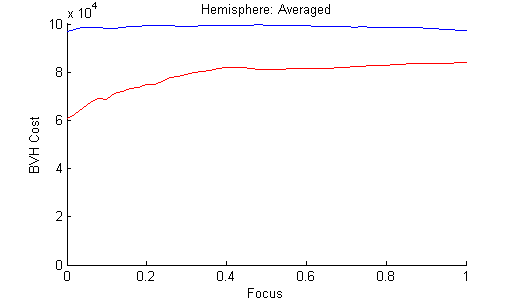
\includegraphics[scale=.3]{hemisphere_average.png}
&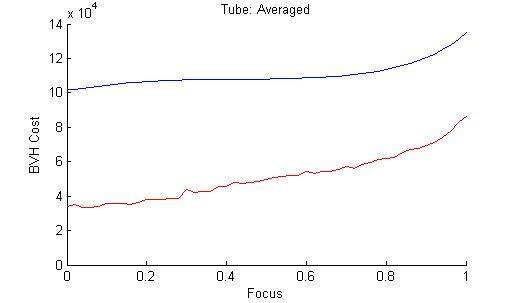
\includegraphics[scale=.3]{tube_average.png} \\
\hline
\end{tabular}
\end{figure*}

\section{Conclusion and Future Work}

\end{document}